\documentclass[10pt]{article}
\usepackage{tikz}
\usetikzlibrary{shapes.misc}
\usepackage[margin=0cm]{geometry}
\pagestyle{empty}
\tikzstyle{every node}=[cross out, draw, red]

\begin{document}

\vspace*{\fill}
\begin{center}
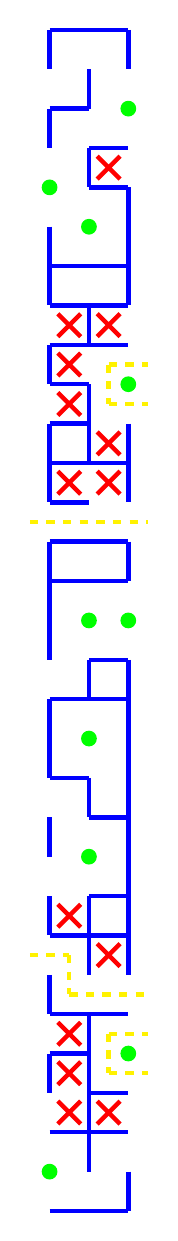
\begin{tikzpicture}[x=0.5cm, y=-0.5cm, ultra thick, blue]
% Walls
    \draw (0,0) -- (2,0);
    \draw (0,2) -- (1,2);
    \draw (1,3) -- (2,3);
    \draw (1,4) -- (2,4);
    \draw (0,6) -- (2,6);
    \draw (0,7) -- (2,7);
    \draw (0,8) -- (2,8);
    \draw (0,9) -- (1,9);
    \draw (0,10) -- (1,10);
    \draw (0,11) -- (2,11);
    \draw (0,12) -- (1,12);
    \draw (0,13) -- (2,13);
    \draw (0,14) -- (2,14);
    \draw (1,16) -- (2,16);
    \draw (0,17) -- (2,17);
    \draw (0,19) -- (1,19);
    \draw (1,20) -- (2,20);
    \draw (1,22) -- (2,22);
    \draw (0,23) -- (2,23);
    \draw (0,25) -- (2,25);
    \draw (0,26) -- (1,26);
    \draw (1,27) -- (2,27);
    \draw (0,28) -- (2,28);
    \draw (0,30) -- (2,30);
    \draw (0,0) -- (0,1);
    \draw (0,2) -- (0,3);
    \draw (0,5) -- (0,7);
    \draw (0,8) -- (0,9);
    \draw (0,10) -- (0,12);
    \draw (0,13) -- (0,16);
    \draw (0,17) -- (0,19);
    \draw (0,20) -- (0,21);
    \draw (0,22) -- (0,23);
    \draw (0,24) -- (0,25);
    \draw (0,26) -- (0,27);
    \draw (1,1) -- (1,2);
    \draw (1,3) -- (1,4);
    \draw (1,7) -- (1,8);
    \draw (1,9) -- (1,11);
    \draw (1,16) -- (1,17);
    \draw (1,19) -- (1,20);
    \draw (1,22) -- (1,24);
    \draw (1,25) -- (1,29);
    \draw (2,0) -- (2,1);
    \draw (2,4) -- (2,7);
    \draw (2,10) -- (2,12);
    \draw (2,13) -- (2,14);
    \draw (2,16) -- (2,24);
    \draw (2,29) -- (2,30);
% Pillars
    \fill[green] (2,2) circle(0.2);
    \fill[green] (0,4) circle(0.2);
    \fill[green] (1,5) circle(0.2);
    \fill[green] (2,9) circle(0.2);
    \fill[green] (1,15) circle(0.2);
    \fill[green] (2,15) circle(0.2);
    \fill[green] (1,18) circle(0.2);
    \fill[green] (1,21) circle(0.2);
    \fill[green] (2,26) circle(0.2);
    \fill[green] (0,29) circle(0.2);
% Inner points in accessible cul-de-sacs
    \node at (1.5,3.5) {};
    \node at (0.5,7.5) {};
    \node at (1.5,7.5) {};
    \node at (0.5,8.5) {};
    \node at (0.5,9.5) {};
    \node at (1.5,10.5) {};
    \node at (0.5,11.5) {};
    \node at (1.5,11.5) {};
    \node at (0.5,22.5) {};
    \node at (1.5,23.5) {};
    \node at (0.5,25.5) {};
    \node at (0.5,26.5) {};
    \node at (0.5,27.5) {};
    \node at (1.5,27.5) {};
% Entry-exit paths without intersections
    \draw[dashed, yellow] (1.5,8.5) -- (2.5,8.5);
    \draw[dashed, yellow] (1.5,9.5) -- (2.5,9.5);
    \draw[dashed, yellow] (-0.5,12.5) -- (2.5,12.5);
    \draw[dashed, yellow] (-0.5,23.5) -- (0.5,23.5);
    \draw[dashed, yellow] (0.5,24.5) -- (2.5,24.5);
    \draw[dashed, yellow] (1.5,25.5) -- (2.5,25.5);
    \draw[dashed, yellow] (1.5,26.5) -- (2.5,26.5);
    \draw[dashed, yellow] (0.5,23.5) -- (0.5,24.5);
    \draw[dashed, yellow] (1.5,8.5) -- (1.5,9.5);
    \draw[dashed, yellow] (1.5,25.5) -- (1.5,26.5);
\end{tikzpicture}
\end{center}
\vspace*{\fill}

\end{document}
